\part{Random Number Generators Based On Optoelectronic Chaotic Laser}
\label{Optoelectronic Chaotic Laser}
\chapter{Introduction}
\label{chaotic laser introdution}

Physical RNGs rely on chaotic or stochastic physical processes. Such random number generators are building the random bits from inherently random or chaotic physical process~\cite{security}, for example, radioactive decay~\cite{radio}, chaotic electrical and optical circuits~\cite{circuits}, and so on. The implementations of physical random generators have been limited to much slower rates than PRNGs because of limitation of the mechanisms for extracting bits from physical randomness without degrading statistical properties. Typically 10 Mb/s could be achieved by using electronic oscillator jitter~\cite{oscillator} and 4 Mb/s using quantum optical noise~\cite{dynes:031109}.

Considerable improvements for the rate of chaotic random bits generation have been reached by using a semiconductor laser in the presence of external feedback \cite{mukai85}, a well known setup in chaotic optical systems. The dynamical processes involved in optical systems can indeed be very fast. Moreover, high complexity chaotic dynamics can be practically obtained, whether due to intrinsic complex nonlinear coupling between light and matter interactions in lasers, or due to the presence of a large delay feedback cavity enabling dynamics with large number of degrees of freedom. 

Chaotic optical signal might consist of pulses with a width of few 10ps and with random amplitude and time positions, which provide attractive potentials to easily generate random bits at fast rates. In~\cite{fast}, a first attempt already reached 1.7 Gb/s RNG, the physical randomness originating from two independent chaotic semiconduct lasers. Each laser intensity signal is practically sampled at an incommensurate rate with respect to the individual optical feedback delay times; then a threshold value is set for comparison with each signal level and to obtain a Boolean sequence; lastly the random bit sequence is produced by executing a XOR function between the two Boolean sequences.  More recently, Reidler and colleagues~\cite{ultrafast2009,ultrafast2010} claim that they successfully demonstrated another method in generating random bit sequence from ultra fast optical chaos, at much faster rate.  In such method, the output of a single chaotic laser, with the optical feedback delay time incommensurate with 
the sampling clock frequency, was digitized by an 8-bit analog-to-digital converter (ADC, practically provided by an ultra-fast digital scope).  Then the difference between adjacent, but not nearest, points from the 8-bit digitized time series is performed (it is defined as a pseudo-``derivative'' operation). At last, a few LSBs only of the subtracted samples values are retained to generate the binary sequence. Following that kind of procedure, generation rate as high as 300~Gb/s are claimed.

In this part, the study of using optical signal to generate random binary sequence according to the method proposed by Reidler, is going to be deepen. We propose to apply the same method on the chaotic waveform generated by another class of broadband photonic oscillations, and to analyze the different post-processing steps involved in this method. We will analyze three key factors in the scheme of~\cite{ultrafast2009} and~\cite{ultrafast2010}: the sampling, the difference of distant samples, and LSBs retaining.  





























\chapter{Noise And Chaos Contributions in Fast Random Bit Sequences Generated From Broadband Optoelectronic Entropy Sources}
\label{Noise And Chaos Contributions In Fast Random Bit Sequence Generated From Broadband Optoelectronic Entropy Sources}


We reproduce and adapt, in this chapter, the content of the publication~\cite{submit4}
submitted to 'IEEE Journal of Quantum Electronics'. In this work, on which I was greatly aided by my supervisor in the OPTO team,  we take a critical look on an article claiming surprising generation bit rates using a chaotic 
optoelectronic device.


\section{Method for Random Bit Sequence Generation from an Optoelectronic Signal}
\label{Method for random bit sequence generation}
In this section we describe the physical setup from which we expect to obtain a fast random bit sequence. We also describe the binary sequence extraction method from the continuous time signal generated by the physical setup, as it was formerly proposed in \cite{ultrafast2009,ultrafast2010}.  Additionally, theoretical interpretation and discussion of this extraction method is proposed in terms of basic signal processing and sampling theory. These interpretation and discussion are intended to give insight on the possible mechanisms at the origin of the bit stream randomness quality.
%
\subsection{Setup delivering a broadband optoelectronic signal}
\label{Setup delivering a broadband optoelectronic signal}
%
In order to additionally support our work with experiments on the generation of optical broadband signals, data recorded from physical chaos generator as well as from optoelectronic noise sources, have been studied. These experiments are moreover different from the ones described in \cite{ultrafast2009} and \cite{ultrafast2010}, although they are also originating from optoelectronic devices.

A twofold physical source of entropy has been used (see Fig.\ref{opto_RNG}), both having been tested for their randomness quality. One source (referred as ``Optoelectronic noise'' in Fig.\ref{opto_RNG}) is originating from physical noise sources in the semiconductor laser light generation process (known as RIN: relative intensity noise), in combination with the electronic noise of the photodetector and its integrated electronic amplifier (thermal noise and semiconduction photodiode junction noise, amplified by the noise figure of the electronic amplifier). A comparable (and even cheaper) optoelectronic noise source was also proposed in \cite{li:OL11}.\\
%
On the contrary, the other physical source of entropy is originating from a strongly deterministic process, which was used recently for a field experiment demonstrating (analogue) chaotic optical masking of 10~Gb/s data signals, transmitted over an installed fiber optic link \cite{lavrov:jqe10}. The strong determinism of this entropy source indeed enabled to implement accurate broadband chaos synchronization at the receiver, in order to remove the chaotic masking signal and thus to retrieve the original binary data stream.  The dynamics of the electro-optical phase chaos generator is ruled by a nonlinear dual delay differential equation implemented in an optoelectronic and electro-optic feedback loop. 

Each of these two signals obtained from noise or chaotic optoelectronic systems, has been processed by using the method proposed in \cite{ultrafast2009}. By doing so, the aim is to support our signal processing analysis on the extraction method of the bit sequence, which is inferring that in both cases, the randomness quality must be very similar. More precisely, we claim that the actual binary sequence randomness is mainly related to the non-deterministic small background noise, and not to the deterministic large amplitude chaotic component.
%
\begin{figure}
  \centering
  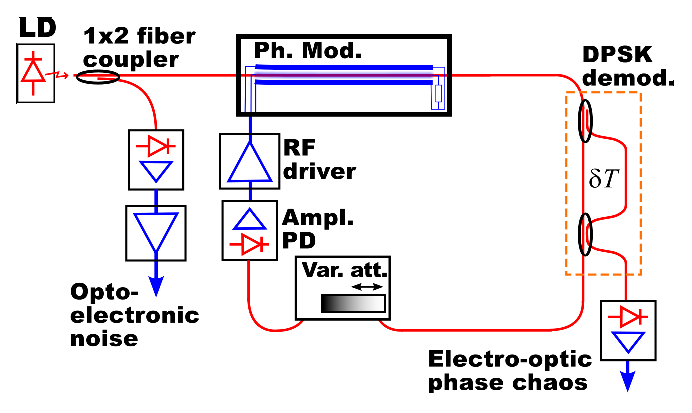
\includegraphics[scale=0.75]{setup_opto_RNG.eps} %[Histogram of
  % digitized laser]
  \hspace{0.5cm}
  \caption{Experimental setup of the optical system used to generate
    signal as physical random sources for the derivation of random bit
    sequences.}
  \label{opto_RNG}
\end{figure}
%
The deterministic chaotic signal can be approximated by the physical solution of a nonlinear dual delay dynamics ruled by the following differential equation:
%
\begin{equation}
  \theta^{-1}\int_0^tx(\xi)d\xi+\tau \frac{dx}{dt}(t)+x(t)=
  \beta\sin^2[x_T-x_{T+\delta T}+\Phi_0],  \label{DDE}
\end{equation}
%
where $x_T$ stands for the delayed signal $x(t-T)$, $\theta$ and $\tau$ are the characteristic times of the low and high cut--off frequency respectively, which are involved in the bandpass feedback filtering of the RF filter. From a signal processing viewpoint, such a dynamical system can be interpreted as a nonlinear delayed feedback oscillator, which is ruled by the dynamics of a linear bandpass filter driven by a nonlinear transformation of two delayed (delays $T$ and $T+\delta T$) versions of the filter output $x(t)$. The chaotic solution signal obtained when the feedback loop gain $\beta$ is high enough (of the order of 5, tuned via the CW laser light intensity), is a white noise like motion covering the full spectral range of the broadband bandpass feedback RF filter, \emph{i.e.}, ca $[30$~kHz$-13$~GHz$]$. This results in a fast noise-like large amplitude signal, which is expected to be suitable for high speed RNG based on a physically generated pseudorandom signal. It is worth noticing that this 
chaotic signal generation process can be viewed as a balanced equilibrium between the RF feedback filter aimed at limiting the spectral span of the signal $x(t)$, and the spectral broadening performed by the nonlinear transformation ($\sin^2-$function of the difference delayed signals $x_T-x_{T+\delta T}$). The offset phase $\Phi_0$ is typically adjusted through the average interference condition physically implemented to provide the $\sin^2$ nonlinear transformation.\\
%
A more accurate description of the generated signal $x(t)$ should also include (small amplitude) noise sources in the equation, the latter noise being actually very similar to the one at the origin of the noisy optoelectronic signal (laser and photodiode noise, also complemented here by the RF electronic amplifier noise). Equation (\ref{DDE}) can however be confidently used solely. On the one hand, it can be used to generate numerically the obtained chaotic motion with qualitative properties that are actually very close to the ones observed in the experiment \cite{lavrov:pre09}; on the other hand it can be used to derive analytically some of the bifurcation features both observed in the experiment \cite{weicker:pre12} and described analytically.
%

\subsection{Extraction method for the random binary sequence}
\label{Design}

\begin{figure}
  \centering
  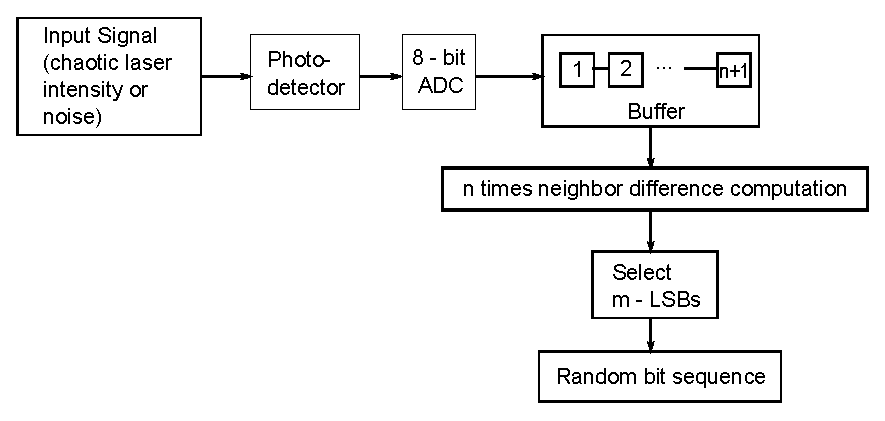
\includegraphics[scale=0.6]{scheme_optic.eps} %[Histogram of
  % digitized laser]
  \hspace{0.5cm}
  \caption{Scheme of the RNG using optical signal}
  \label{derivative}
\end{figure}

%
A schematic view of the algorithm used to extract a random binary sequence from a broadband physical signal, as proposed in~\cite{ultrafast2010}, is depicted in Fig.\ref{derivative}. On the basis of a physical setup delivering a broadband signal, as the one described in the previous section, a real time oscilloscope is firstly involved to perform an analogue to digital conversion of the output signal of the setup. This conversion is typically achieved via an 8-bit digitizer at a sampling rate of 40~GHz. In the next subsection, we will discuss from the signal theory viewpoint some particular processing issues that are suspected to significantly contribute to the actual randomness of the final binary sequence. More precisely, sampling issues will be discussed, quantization issues, and also post-processing operations (such as distant sample difference, and LSB-only retaining). This signal processing is performed before getting the actual final random binary sequence to be tested for their randomness quality via 
standard statistical test suites.
%
\subsubsection{Sampling issues: aliasing for enhanced entropy}
\label{sampling issues}
%
In the following, we assume that samples are originally acquired by a real time digital scope measuring a broadband complex time trace. Such equipment is designed to follow the classical Shannon sampling theorem: the sampling rate $f_\text{S}$ is matching the instrument analogue input bandwidth, which defines the maximum Fourier frequency $f_\text{M}$ that can be captured by the instrument. The Shannon sampling theorem indeed states that a limited bandwidth signal can be digitized without loss of information, when the sampling frequency is at least twice the maximum signal frequency. The sequence of the samples $\{s_n=x(nT),~n\in\mathbb{Z}\}$ can be defined as a function of the continuous time as follows:
%%
\begin{eqnarray}
  \label{eq:sampling1}
  s(t)=x(t)\cdot\cha_{T_\text{S}}(t), \\
  \nonumber \text{where}~\cha_T(t)=\sum_{k=-\infty}^{k=+\infty}\delta(t-k\,T) .
\end{eqnarray}
%%
A typical illustration of the proof for the sampling theorem is presented in Fig.\ref{sampling_th}, as one describes the spectrum of such a sampled signal $s(t)$,
%
\begin{equation}
  \label{eq:S(nu)}
  S(\nu)=\text{FT}[s(t)]=X(\nu)\star \text{FT}[\cha_T(t)]
  =\frac{1}{T}X(\nu)\star \cha_{1/T}(\nu),
\end{equation}
%
where we have used the well-known result that the Fourier Transform (FT) of a comb is also a comb. The convolution product in the Fourier domain reveals that the spectrum of the sampled signal is the result of the superposition of an infinite number of regularly spaced replica of the original signal spectrum $X(\nu)=$FT$[x(t)]$, two neighboring replica being separated by the sampling frequency $f_\text{S}=1/T$. Thus, if the maximum frequency $f_\text{M}$ of the bounded support of $X(\nu)$ is less than $f_\text{S}/2$, the replicated spectra do not overlap (see Fig.\ref{sampling_th}(a)). It is then obvious that a suitable window filtering of the sampled signal $s(t)$ allows to recover in the Fourier domain exactly the same spectrum than the one of the original signal $x(t)$ (\emph{e.g.}, a filter transmitting perfectly all the Fourier components in a frequency band such as $[-f_\text{S}/2,+f_\text{S}/2]$, and rejecting all the other Fourier components for the other frequency ranges).
%
\begin{figure}
  \centering
  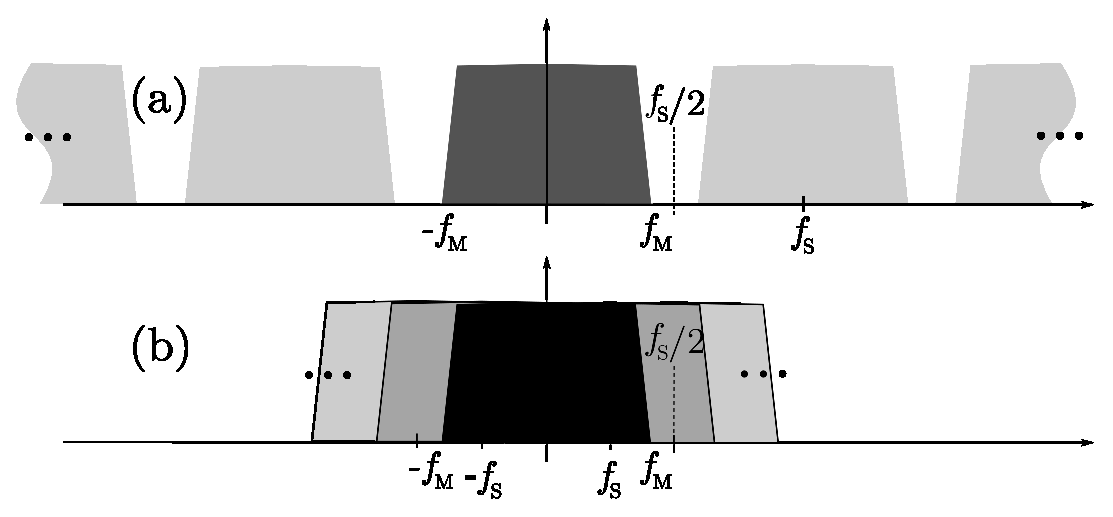
\includegraphics[width=0.45\textwidth]{sampling_th.eps}
  \hspace{0.5cm}
  \caption{Illustration of the properly fulfilled sampling theorem
    conditions (a), and the incorrect sampling condition leading to
    aliasing (b).}
  \label{sampling_th}
\end{figure}
%
When undersampling is used, the {\em aliasing} phenomenon occurs in the Fourier domain. It consists then of overlaps between the replicated spectra due to the comb convolution. The actual spectrum of the sampled signal $s(t)$, can be viewed as a complex mixing of the frequency components of the original signal $x(t)$, due to the overlapped replica of $X(\nu)=$FT$[x(t)]$.
%
\begin{figure*}
  \centering \subfigure[]{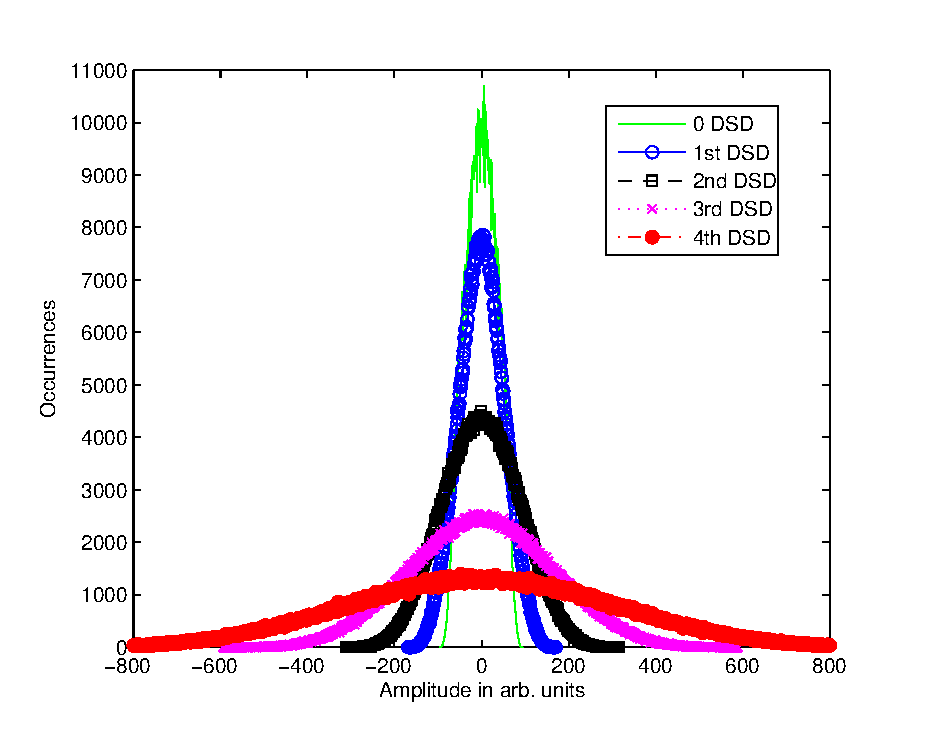
\includegraphics[scale =
    0.5]{chaos_derivative.eps}} \subfigure[]{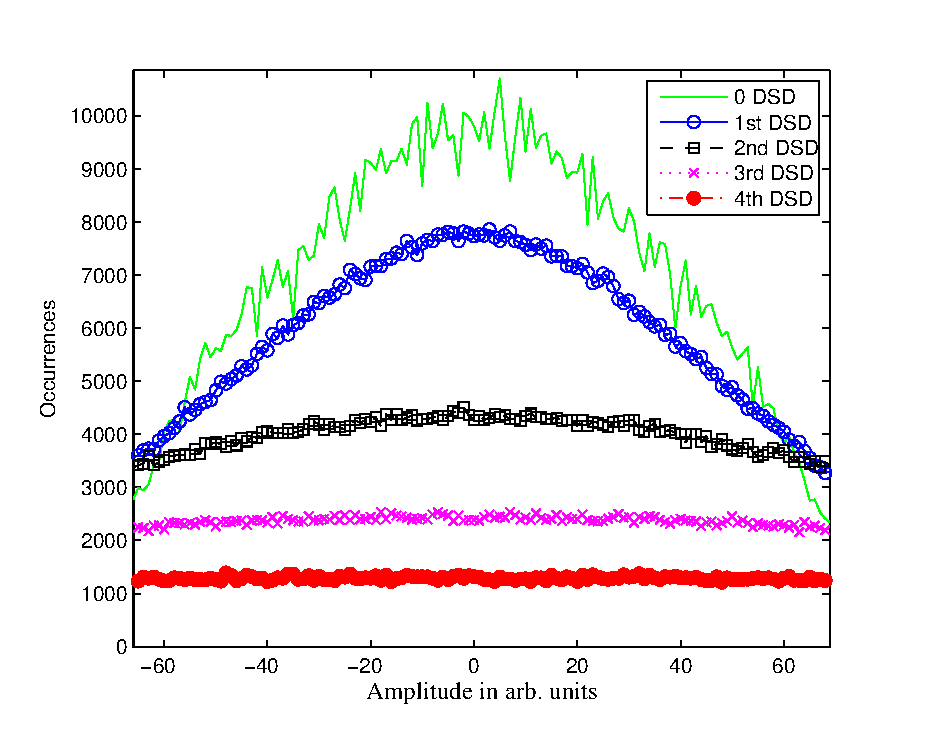
\includegraphics[scale =
    0.5]{chaos_derivative_zoom.eps}}
  \subfigure[]{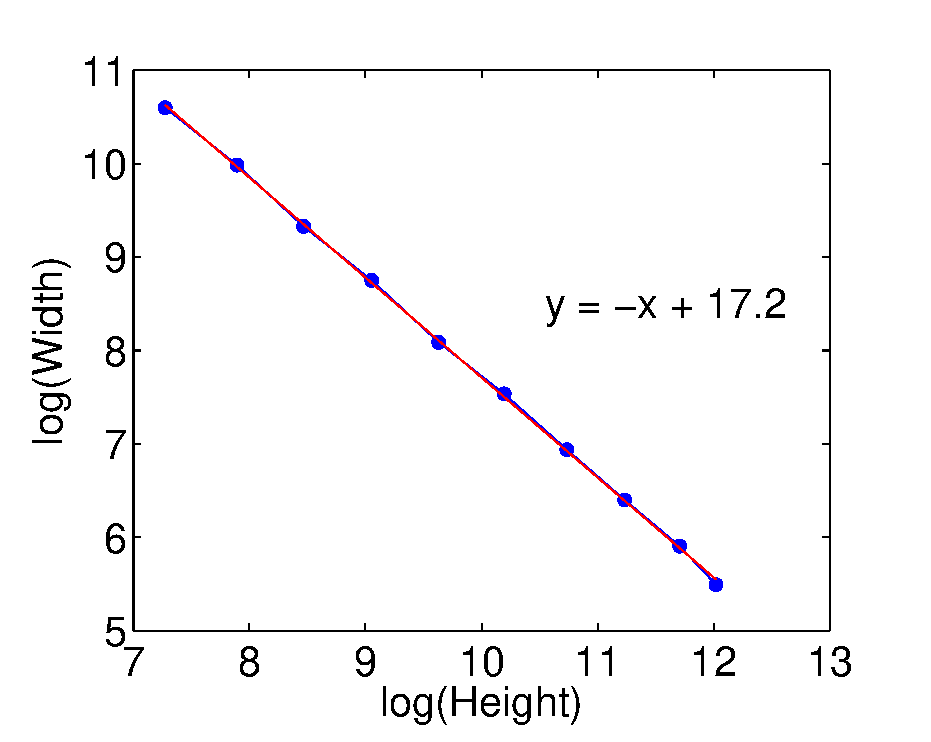
\includegraphics[scale = 0.5]{cwh.eps}}
  \caption{(a) For $1$st-$4$th times DSD for chaotic laser intensity
    sampled by $2.5$GHz ADC; (b) Zooming of the centering area of (a);
    (c) For 1st-10th times DSD, the log-log plot between weight and
    height, showing the hyperbolic relationship between the two as DSD
    is repetitively processed.}
  \label{diff of chaos}
\end{figure*}
%
The procedure of selecting only one sample every $n$ from the original
sampled sequence, is thus equivalent to an aliasing operation with an
undersampling of order $n$. The original goal of cementification of
the extracted sample sequence, can thus be viewed as an aliasing
technique resulting in a complex mixing of the original frequency
components. The consequence is an increased entropy of the output
sequence, as this procedure, when viewed in the time domain, results
in the vanishing of the short time correlations. On the contrary,
these short time scales correlations are necessarily present when the
conditions of the sampling theorem are fulfilled. Another consequence
is that such an operation is unidirectional, in the sense that
original information is actually lost after an aliasing process.
Because of the complex mixing of the Fourier frequency components, the
original spectrum cannot be recovered with a ``simple'' unmixing.

\begin{figure*}
  \centering \subfigure[]{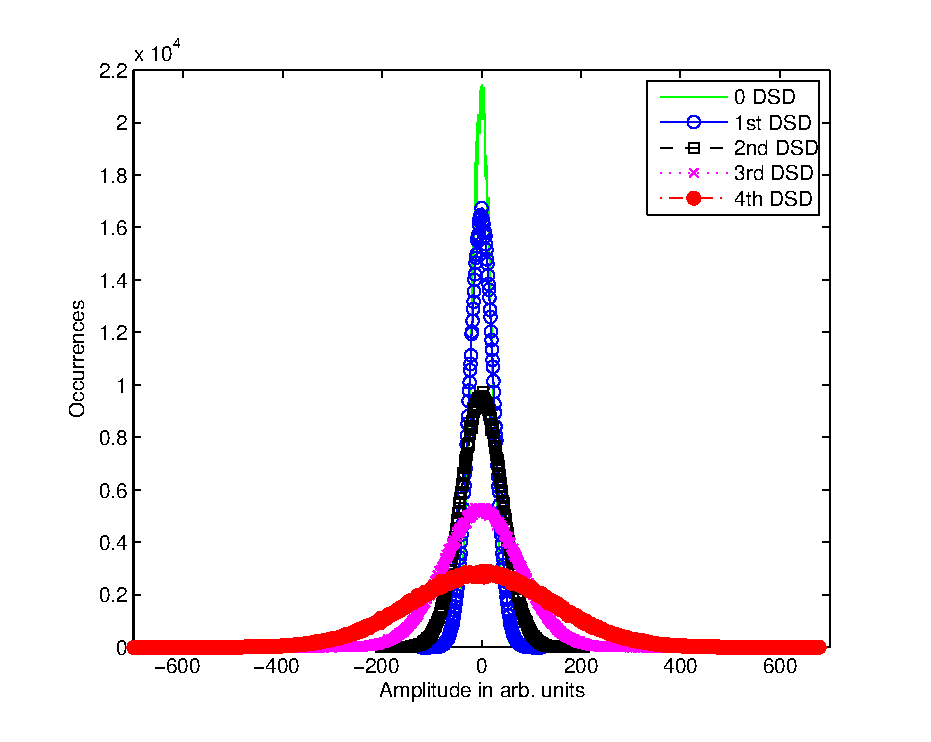
\includegraphics[scale =
    0.5]{noise_derivative.eps}} \subfigure[]{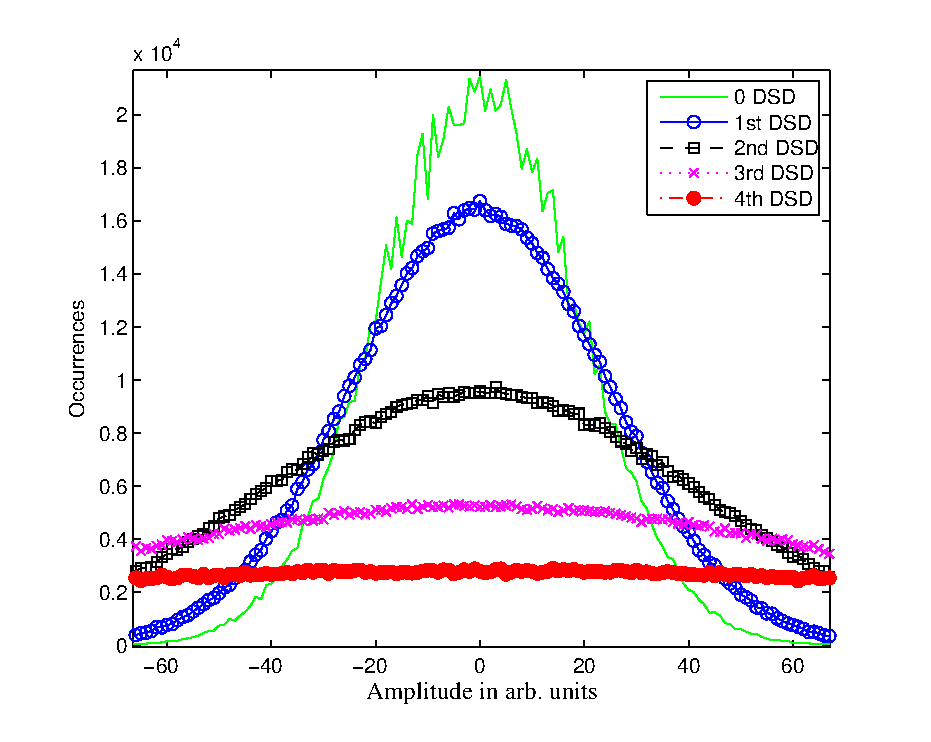
\includegraphics[scale =
    0.5]{noise_derivative_zoom.eps}}
  \subfigure[]{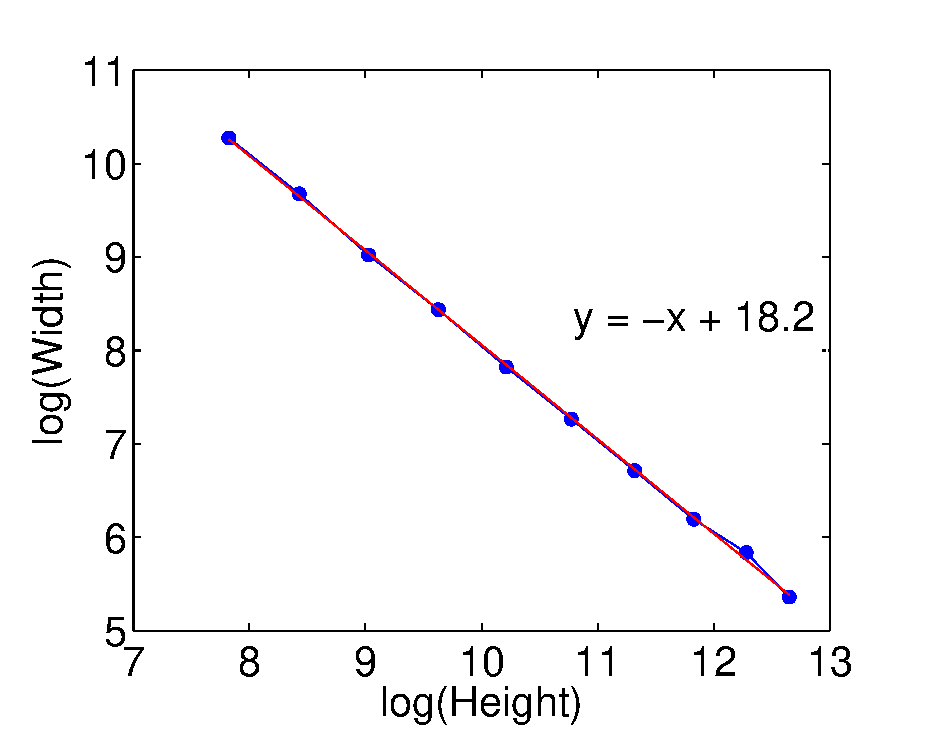
\includegraphics[scale = 0.5]{nwh.eps}}
  \caption{(a) For $1$st-$4$th times DSD for noisy signal sampled by
    $2.5$GHz ADC; (b) Zooming of the centering area of (a); (c) For
    $1$st-$10$th times DSD, the log-log plot between weight and
    height, showing the hyperbolic relationship between the two as DSD
    is repetitively processed.}
  \label{diff of noise}
\end{figure*}

\subsubsection{Further post-processing: difference sequence between
  distant samples}
\label{dsd}
%
In~\cite{ultrafast2009} and~\cite{ultrafast2010}, computing the
difference sequence between two neighbor samples are named as
``derivative''. However, mathematically speaking, the term
``derivative'' of $x(t)$ is used for the asymptotic value $(
x(t+\Delta t)-x(t) )/ \Delta t$ when $\Delta t\rightarrow 0$. In the
physical case of a finite sampling rate, the neighbor samples are
obviously not infinitely close in time, hence we prefer not to use
``derivative'' here. More precisely, we are dealt here with
significantly separated samples in time, since strong aliasing is
first operated (see Section~\ref{sampling issues}), with an
undersampling number up to $n=16$. The initial 40~GHz sampling rate is
respecting the oscilloscope analogue input bandwidth of 12~GHz, but
the final series obtained after retaining 1 sample over 16, is
corresponding to a 2.5~GHz undersampling rate. The samples obtained
after this distant sample difference (which will be called later DSD)
operation can thus be described as follows:
%
\begin{equation}
  \label{eq:diff_samples}
  \{d\,_k^n\}_{k\in\mathbb{N}} = \{x[k\,T]-x[(k-n)T],
  k\in\mathbb{N}\}.
\end{equation}
%
If we try again to analyze in the Fourier domain the meaning of this
second processing, one obtain the following expression for the Fourier
spectrum of $n-$undersampled difference signal:
%
\begin{equation}
  \label{eq:n-diff_spectrum}
  D(\nu) = \left[2\,i\,e^{-i\pi\nu nT}\, X(\nu)\sin(\pi\nu
    nT)\right] \star\cha_\frac{1}{nT}(\nu).
\end{equation}
%
This expression reveals a so-called channeled spectrum filter, which
applies a periodic sinusoidal modulation of the original spectrum
$X(\nu)$. One could notice that the maximum transmission of this
filter is centered at half the undersampling rate ($(nT)^{-1}/2$)
where aliasing is maximally symmetric (thus somehow selecting the
frequency components that are most affected by aliasing), and the zero
transmission frequencies are centered at zero and $\pm(nT)^{-1}$
(where the aliasing phenomenon is the less pronounced in the Fourier
spectrum, as long as $n$ is not too large). When focusing on the low
frequency domain only, another comment about the action of this DSD
processing could be made: the very low frequencies are filtered out,
which consequence is to asymptotically set to zero the mean value of
the corresponding sample set, and thus also improving the symmetry
around zero of the amplitude probability distribution.

The Fourier analysis of the DSD processing is however not as obvious
as for the aliasing issue in terms of randomness enhancement, or
entropy amplification. A more meaningful discussion can however be
made through the analysis of the statistical sample distribution of
the DSD compared to the original one. More precisely, Fig.\ref{diff of
  chaos}a shows the evolution of the amplitude statistics when the DSD
processing is iterated several times. One clearly sees that the
statistics is more and more symmetric resembling closer and closer to
a Gaussian distribution. This effect can be qualitatively explained
through the analysis of the DSD principle. Since the difference is
performed between the same sample sequence but shifted in time over a
quantity large enough compared to the correlation time, one can
interprete the DSD as the superposition of nearly independent
pseudorandom processes. The central limit theorem can then be used to
explain qualitatively the amplitude distribution convergence towards a
Gaussian one (limit of the amplitude distribution for the
superposition of an asymptotically large number of independent random
processes).\\
At the same time, as more and more DSD are operated, the amplitude
range is increased along the horizontal axis, whereas the maximum of
the statistics along the vertical axis is inversely decreased.  Figure
\ref{diff of chaos}c shows the numerical evidence of a hyperbolic
relation between width and height for the successive iterated
processings. Last but not least, the analysis of the statistics
evolution of the sample amplitude after a few iterations of the DSD
processing, allows one to realize one of the main properties for the
last post-processing operation proposed in
\cite{ultrafast2009,ultrafast2010}, and leading to the final random
bit sequence: LSBs only retaining.


\subsubsection{LSB retaining, and intrinsic noise of the original
  sequence}

When one keeps the LSBs only of the samples obtained after a few DSD
processing, this means that only the small amplitudes are
considered. Zooming in Fig.\ref{diff of chaos}b into the small
amplitude range, \emph{i.e.}, into the origin of the corresponding
statistical histogram, one clearly sees that the statistics becomes
nicely flat, thus resembling to a uniform distribution when
considering the LSBs
only.\\
A straightforward issue can then be raised about the actual source of
randomness leading to the final bit sequence, as reported in
\cite{ultrafast2009,ultrafast2010}. This source of randomness has been
practically attributed to the chaotic solution generated by the
original physical system, a SC laser diode subjected to proper optical
feedback, under such conditions that chaotic motion is
obtained. However, since only LSBs are retained in the final step of
the random bit sequence extraction method, one is allowed to question
about the actual influence of the always present background noise
(physical noise, but also quantization noise due to the analogue to
digital conversion of the fast digital scope instrument serving as the
ultra-fast acquisition device). This background noise is indeed a
small amplitude compound of the acquired signal, and as such, it
should have a potentially important influence on the small amplitude
fluctuations represented by the LSBs.

To investigate this issue, we performed a similar analysis as the one
done in the previous subsections on the chaotic motion of a nonlinear
electro-optic delay dynamics, but with a physical signal a priori
originating from physical and digital noise sources only, without any
deterministic chaotic compound. This signal is chosen to be the output
of the amplified photodiode of the same setup, but without the
nonlinear delayed feedback loop at the origin of the chaotic time
series: the amplified photodiode signal is issued from the laser
intensity noise, it comprises also the photodiode junction noise and
the electronic amplifier noise (see ``Optoelectronic Noise'' output in
Fig.\ref{opto_RNG}). Although the electrical signal level is
significantly lower, we used the scope magnification to get a time
trace of a comparable amplitude with respect to the scope vertical
amplitude range, thus resulting in an effective digital scope
quantization over a comparable number of bits with respect to the
chaotic signal. Out of the physical noise sources (laser intensity
noise, photodiode and electronic amplifier noise), we also have the
digitization noise. The latter is typically evaluated by the scope
manufacturer through an equivalent number of quantization bits when
taking into account all the noise contributions involved in the
digitization process. This number of effective bits is 5 to 6, meaning
that the number of bits that are strongly influenced by the
acquisition procedure is at least 2 (the 2 LSBs in the original time
series recorded by the scope).

We have reported in Fig.\ref{diff of chaos} and Fig.\ref{diff of noise}
the statistics evolution of the digitally acquired optoelectronic
noise signal and its width / height evolution. The figures clearly
show very similar features. From this rough analysis of the influence
of the two physical signals (the optoelectronic noise and the
electro-optic chaos), we realize that the post-processing leads to
qualitatively equivalent final bit sequence. This observation, and the
previous analysis of the post-processing steps, support the
assumption, at least qualitatively, that the randomness of the final
bit sequence might be mainly issued from the post-processing
steps. The chaotic feature of a time series appears then as actually
not required for the generation of a random bit sequence, when the
latter generation process is performed according to the described
post-processing operations: aliasing through undersampling of the
original acquired time series, DSD processing, and LSBs retaining.

\section{Effect of Noise on the Entropy Rate in the Binary Sequence}
\label{entropy}
%
In this section, the time evolution of the entropy in the final binary
sequence is evaluated under different choices for the method used to
build the final random bit stream from the chaotic signal. The aim is
to get insight in the origin of the entropy creation mechanism
involved in the construction of the final random bit stream. More
precisely, we aim at discriminating under which conditions the
deterministic feature of the chaotic signal (the determinism coming
from the dynamics described by Eq.(\ref{DDE})) is indeed involved in
the entropy of the extracted bit stream. To achieve this goal we
reproduce the method proposed in \cite{PhysRevE.85.016211}, which is
intended to measure the sensitivity to initial condition (SIC) of the
deterministic chaotic motion in the presence of additional small
noise. This measure consists in calculating the temporal entropy
evolution for the generated binary random sequence, with respect to
several different noise realizations.
%
\subsection{Introducing noise in the simulated chaotic dynamics}
%
For the entropy calculation, we first consider a transient-free
chaotic solution of Eq.(\ref{DDE}) ($\beta=5$). To achieve such a
solution, Eq.(\ref{DDE}) is integrated under the proper parameter
conditions known to lead to a high complexity chaotic solution. This
preliminary numerical integration is performed over a duration long
enough compared to the slowest characteristic time scale of the
dynamics ($\theta$), so that the asymptotic trajectory is free of any
transient. Once this corresponding chaotic attractor is supposed to be
reached via the numerical integration, this asymptotic solution can be
associated to a single temporal waveform covering only the longest
time delay of the dynamics, i.e. $T+\delta T$: this is defining the
initial condition of the corresponding delay based, and noise-free,
chaotic dynamics, from which noise influence will be explored. We then
introduce in the right hand side of Eq.(\ref{DDE}) an arbitrary small
additive noise term (small perturbation along the chaotic
trajectory). The noise amplitude is arbitrarily set so that the
Signal-to-Noise Ratio (SNR) is 40~dB. After further integrating
Eq.(\ref{DDE}) with the noise term and starting from the initial
condition corresponding to the calculated noise free chaotic
trajectory, one is able to obtain a continuously noise-perturbed
chaotic trajectory. When repeating this calculation with several
different noise realizations, one then expects to observe the effect
of SIC when comparing the different noise perturbed chaotic
trajectories. This property manifests itself through a progressive
amplification (as time is running) of the small perturbations
materialized by the added noise. Comparing the different calculated
waveforms, they consequently looks all the same right after the noise
addition, but they split apart (differently for each pair of such time
series) after a typical time scale related to the inverse of the
largest Lyapunov exponent of the chaotic dynamics (see
Ref.\cite{PhysRevE.85.016211} for details). Two such simulated
waveforms are represented in Fig.\ref{noise_chaotic_signal}, after the
undersampling procedure, and before the DSD and bit retaining
processes for the final extracted binary sequence. The waveforms thus
do not appear anymore as continuous in time due to undersampling. For
these two realizations and with the chosen SNR for the noise
amplitude, one clearly sees that the two time series separated one from
each other after a typical time scale of ca. 300~ns. This time scale
is of the order a few tens of the largest time delay $T+\delta T$,
which is corresponding to a few tens round trips of the chaotic signal
in the nonlinear delayed feedback loop. This is fully consistent with
the typical order of magnitude of the inverse largest Lyapunov
exponent, i.e. it is of the order of the largest time delay in the
dynamics.
%
% the statistics subjected ne thus consider two different noisy time
% series added to the same initial chaotic dynamics, one obtains two
% resulting time series that are very close right after the origin of
% time (when small noise starts to be added to the chaotic
% trajectory), but that are progressively more and more split apart
% after the time needed to amplify the noise up to the level of the
% original chaotic amplitude. This is illustrated in
% Fig.\ref{noise_chaotic_signal}, where we have represented the
% subsampled (2.5~GHz) amplitudes, obtained after integration of
% Eq.(\ref{DDE}) with two different added noise sequences (but with
% the same SNR). For these two realizations and with the chosen SNR
% for the noise amplitude, one clearly sees that the time series
% separate after a typical time scale of 300~ns, of the order a few
% tens of the largest time delay $T+\delta T$ (thus corresponding to a
% few tens round trips of the noise perturbed initial condition in the
% nonlinear delayed feedback loop oscillation process).

% In order to compare the value of noise strength corresponding to the
% noise level observed in experiments, Signal-to-noise ratio (often
% abbreviated SNR or S/N) is applied. SNR is a measure used in science
% and engineering that compares the level of a desired signal to the
% level of background noise. It is defined as the ratio of signal
% power to the noise power. In decibels, the SNR is defined as

% \begin{equation}
%   \label{snr2}
%   SNR_\text{dB} = 10(\log_{10}{A_\text{signal}^2} - \log_{10}{A_\text{noise}^2})
% \end{equation}
% where $A$ is root mean square (RMS) amplitude.

% The model of Section~\ref{Setup delivering a broadband
% optoelectronic signal} is used.
%
\begin{figure}
  \centering
  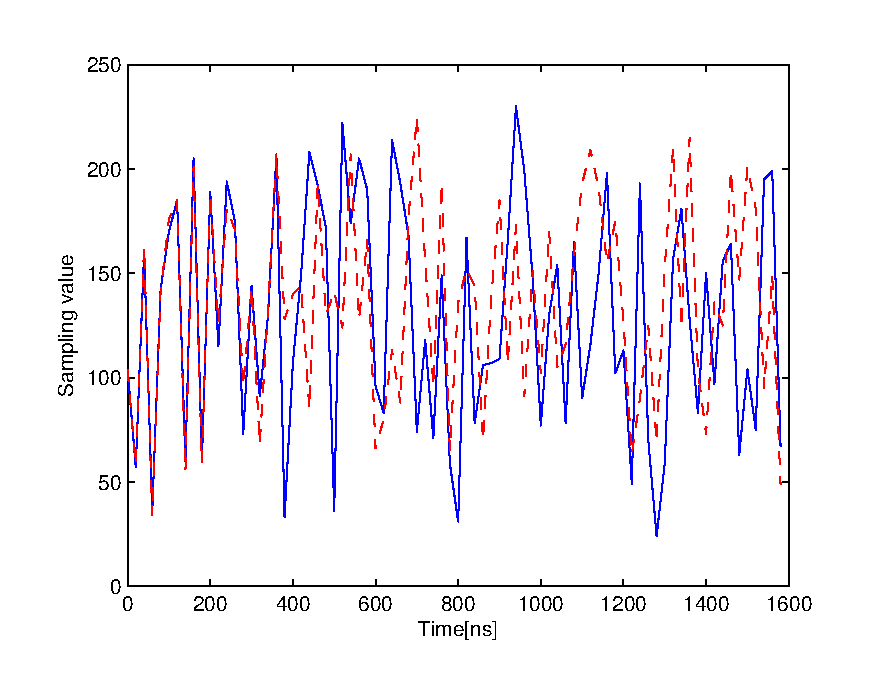
\includegraphics[width=0.8\textwidth]{chaos_noise.eps}
  \hspace{0.5cm}
  \caption{Two temporal waveforms of chaotic laser intensity starting
    from the same initial conditions with different noise sequences
    added at time $0$. The noise amplitude is set so that SNR is 40~dB
    (the signal energy being calculated on the noise-free chaotic
    trajectory)}
  \label{noise_chaotic_signal}
\end{figure}
%
\subsection{Entropy estimation for each bit cell}
%
% The entropy rate is then evaluated as follows. For $N$ many
% different realizations of such noise-perturbed chaotic time series
% which are starting wth the same initial conditions, one can extract
% as many $N$ random binary sequences according to a fixed bit
% extraction method. This allows one to compute, at every time $t_k$
% for which a new bit is extracted, the probability distribution of
% zeros and ones, $p_0(t_k)$ and $p_1(t_k)$ respectively. The
% statistical entropy is then simple simply evaluated as .
%
Many different noisy chaotic time series ($N=10^3$) are simulated to
generate as many random bit sequences. Each realization is calculated
from the same initial conditions (the noise free chaotic waveform over
one largest delay time interval), but with different added small noise
perturbations. From each obtained time series, one can explore various
bit stream extraction methods, e.g. with or without DSD, or even with
several successive DSD processing, with the LSB retaining or with the
MSB, \ldots For a fixed bit extraction method, the $N$ obtained bit
sequences can be used to calculate, at each time $t_k$ of a new
extracted bit, the probabilities $P_0(t_k)$ and $P_1(t_k)$ for
obtaining a bit 0 or 1 respectively. This time varying probability
distribution is then used to calculate how the statistical bit entropy
evolves in time,
%
\begin{equation}
  \label{entropy_compute}
  H(t) = -\sum^1_{i=0}\,P_i(t)\cdot\log_2P_i(t).
\end{equation}
%
As described in \cite{PhysRevE.85.016211} if SIC of a chaotic dynamics
is indeed involved in the final bit sequence, the $N$ extracted bit
sequences are initially strongly correlated. This is because the bits
are originating from the same initial chaotic waveform. Consequently,
the influence of the small added noise is negligible at the initial
times of the deterministic chaotic dynamics: the entropy at small $t$
is expected to be close to zero if indeed the dominating phenomena is
deterministic. However, as time is evolving, SIC is amplifying the
influence of the small noise amplitude on the large amplitude chaotic
motion, and the $N$ bit streams realizations are more and more
decorrelated, leading progressively to a maximum binary entropy of
1. This unity entropy means an equal probability for obtaining bit
zero and one, independently of any deterministic motion. The influence
of the small added noise term is then dominating the output random bit
stream.
%
\begin{figure*}
  \centering
  \subfigure[]{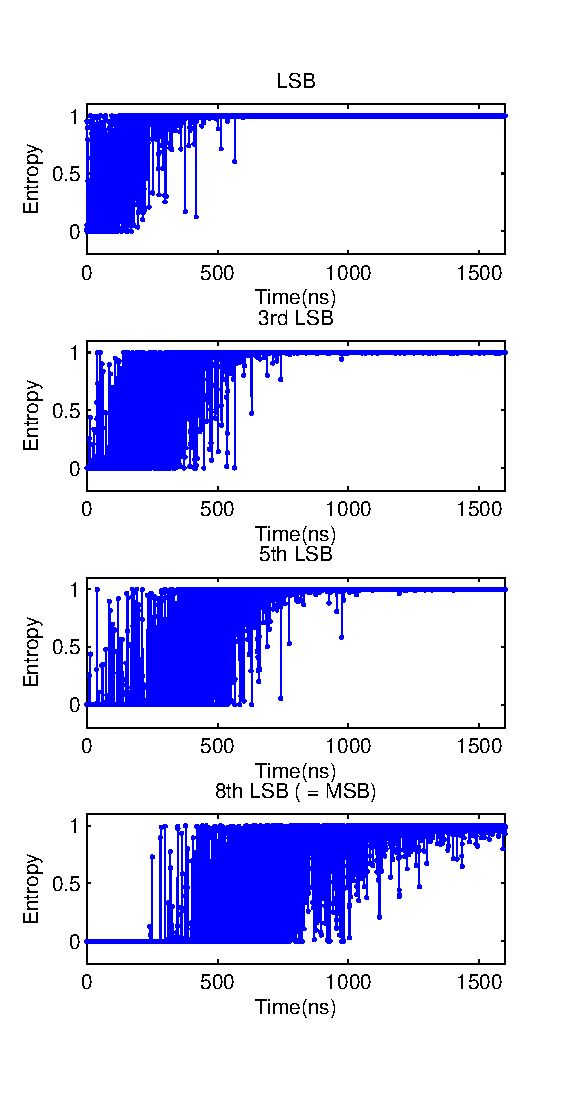
\includegraphics[width=0.32\textwidth]{entropy_value_lsb_msb_40ghz.eps}}
  \subfigure[]{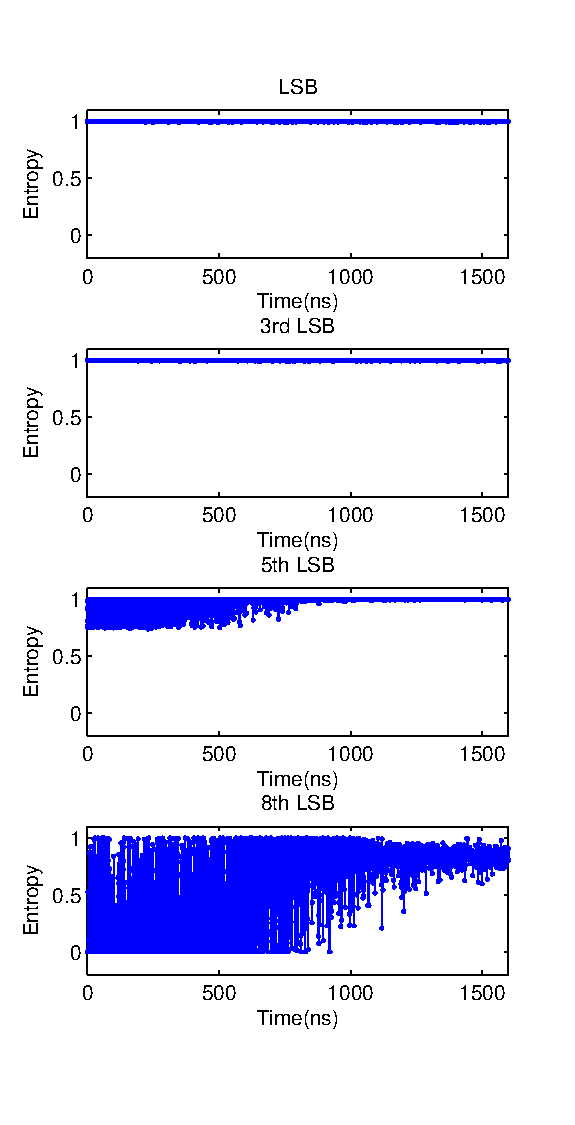
\includegraphics[width=0.32\textwidth]{entropy_value_lsb_msb_40ghz_d1.eps}}
  \subfigure[]{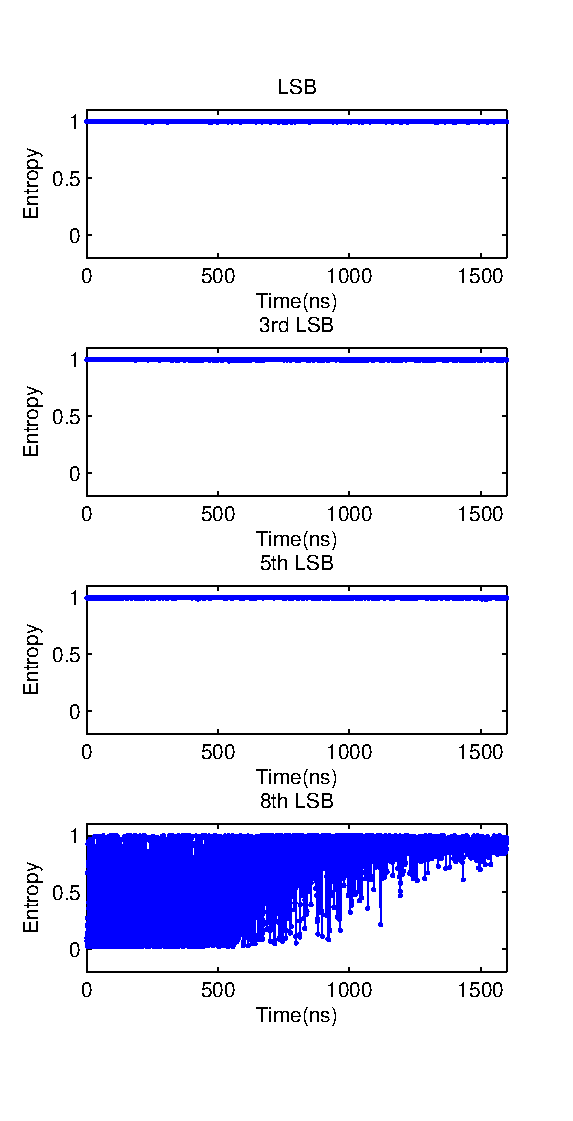
\includegraphics[width=0.32\textwidth]{entropy_value_lsb_msb_40ghz_d2.eps}}
  \caption{Some LSBs entropy as a funtion of time for an ensemble of
    time t = 0. The noise strength is $-40$~db, with sampling rate
    $2.5$ GHz $8$-bit ADC. (a) For sampling value; (b) For the 1st DSD
    of the sampling value. (c) For the 2nd DSD of sampling value.}
  \label{entropy_signal_lsbmsb}
\end{figure*}
%

Figure \ref{entropy_signal_lsbmsb} represents the obtained binary
entropy calculated with different bit extraction methods. In the first
row, the binary entropies obtained from a direct 8-bits ADC for
different bits from LSB to MSB, are plotted as a function of
time. According to the description of~\cite{PhysRevE.85.016211},
memory time is defined as the time required for the entropy to reach a
value close to one. One clearly sees that as the bits chosen for the
random bit stream moves from LSB to MSB, the memory time of the
related bit cell is increasing. This illustrates that MSB is more
withstand in the random bit creation process compared to
LSB. Differently speaking, the small noisy compound in the chaotic
signal is positively influencing randomness quality of the bit stream
when extracted from the LSB. On the contrary MSBs that are related to
greater amplitudes of the chaotic motion, do have a strong
deterministic origin. One has to wait for the memory time before MSBs
can also lead to a good quality random bit stream. This gives an
explanation already drawn in Section~\ref{Design}, that LSBs are more
suitable for fast random bit sequence generation, because they exhibit
a shorter memory time. One could also say that the speed efficiency in
the random bit sequence generation process is better with the LSB
retaining method, because mostly small amplitude noise is actually
involved without any deterministic origin.\\
Figure \ref{entropy_signal_lsbmsb} also reports on the entropy
creation in time, when one or more DSD processing is used. This is
represented in the second and third column of the figure. The
contribution of DSD clearly appears in the entropy rate. DSD is
shortening the memory time, thus speeding up the possible rate at
which actually ``good'' randomness quality can be obtained. Even when
intermediate bit cells are used (e.g. 5th LSB, and twice DSD), a
perfect unity entropy is already achieved at the very first time. An
interpretation could be that DSD is amplifying the non deterministic
small noise influence, and thus is attenuating the detrimental large
amplitude determinism.\\
The conclusion on Fig.\ref{entropy_signal_lsbmsb} is that fastest
entropy rate (down to the actual sampling) can be achieved when LSBs
are used, and when several DSD processing are performed. This
corresponds to the plots on the upper right positions, for which unit
entropy is already achieved very close to the time origin. On the
contrary, the MSBs are showing a non-zero memory time, meaning that
higher entropy for good randomness quality can only be obtained if
slower undersampling is used. Two successive bits would need to be
separated by the memory time in order to get a good randomness quality. The worst
conditions are shown in the lower left plots, with MSBs and without
DSD processing. One could notice that MSB is actually equivalent to
the 1-bit ADC used in \cite{fast}, where we can suspect that the
deterministic chaotic motion plays indeed a crucial role in the final
random bit stream instead. On the opposite, the LSB retaining method
of \cite{ultrafast2009} makes use of the small background noise
present in the chaotic time trace, with a probably small or negligible
contribution of any deterministic chaos origin.

Fig.\ref{lsb2msb_entropy} shows the plots of every bit cell entropy
averaged over $10^3$ trajectories.  Each plot of entropy is obtained
as a function of time for an ensemble of time series starting with
exactly the same initial condition at time $t = 0$. Eight plots are
shown in Fig.\ref{lsb2msb_entropy} corresponding to eight different
position bit cell of the value. These curves are the smoothed
versions, due to averaging, of the curves represented in the first
column of Fig.\ref{entropy_signal_lsbmsb}. Again, it can be seen that
more time is required to converge to a unity entropy when using MSB
compared to the use of LSB. Differently speaking, the memory time
depends on bit cell selecting, MSB and LSB appearing as the slowest
and fastest entropy increasing rate, respectively.

%
\begin{figure}[h]
  \centering
  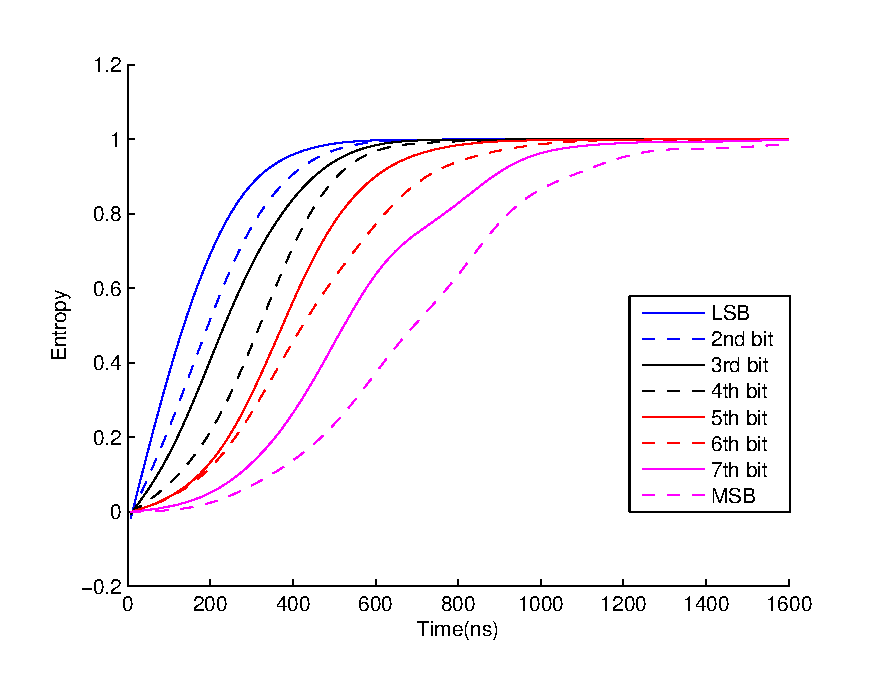
\includegraphics[width=0.5\textwidth]{lsb2msb_entropy.eps}
  \caption{Averadge growth of bit entropy and its dependence on bit
    cell selecting (from MSB to LSB)}
  \label{lsb2msb_entropy}
\end{figure}


\section{Statistical Tests}
\label{comparison}
%
Additionally to the previous signal theory analysis of the processing
steps used in the bit extraction method, this section is intended to
qualify the final bit stream in terms of their benchmarking from
several standard randomness test suites. We thus verify in this
section that the analyzed and used method proposed in
\cite{ultrafast2009} and \cite{ultrafast2010} have led also in our
experiment to quasi-equivalent random bit stream quality, whether from
the deterministic EO phase chaos generator or with the optoelectronic
noise source.
%
% is proposed, the chaotic laser intensity and noisy signal generation
% are setup as Fig.\ref{opto_RNG}, $8-$bit ADC are using to sample the
% signal at 40~GHz clock.
%
%
\subsection{The tested streams}
%

First of all, we give here a brief description of the tested methods
that have been formerly proposed in~\cite{ultrafast2009} and
\cite{ultrafast2010}.

On the one hand, in~\cite{ultrafast2009}, authors have used a DSD
method to generate a random bits stream. The chaotic laser signal is
sampled by using a $2.5$ GHz ADC, and then $5$ LSBs of every first DSD
value are joined together to generate the final random sequence.  On
the other hand, in~\cite{ultrafast2010}, the chaotic laser signal is
sampled thanks to a $20$ GHz ADC. Then the DSD operation is processed
$4$ times and $8$ LSBs of each value are joined to produce the
pseudorandom bit stream.

These two schemes are both adapted to optoelectronic noisy signal. The
generated streams sourced from chaotic laser and noise are compared by
standard statistical tests in the next subsections.

\subsection{Statistical tests}
%
%Considering the properties of binary random sequences, 
We have previously shown that various
statistical tests can be designed to evaluate the assertion that a given
sequence is generated by a perfectly random source. In this section, we have performed
some statistical tests on the optoelectronic noise and electro-optic
chaos generators considered here. These tests include NIST
suite~\cite{Barker05recommendationfor}, DieHARD battery of tests~\cite{Marsaglia1996}, ENT
program~\cite{ent}, and Comparative test parameters. 
%A brief
%description of each of the aforementioned tests is given in the
%following paragraphs.

\subsubsection{NIST statistical test suite}

In Tab.\ref{nist}, the random streams generated by the chaotic laser
and by the noisy signal have both obtained a $100\%$ passing rate when
considering the NIST battery of tests, thus it is impossible to found
a difference between the two streams using the NIST suite.


\begin{table*}[!t]
  \renewcommand{\arraystretch}{1.3}
  \caption{NIST SP 800-22 test results ($\mathbb{P}_T$)}
  \label{nist}
  \centering
  \begin{tabular}{l|c|c|c|c}
    \hline
    Method & \multicolumn{2}{c|}{$2.5$GHz, $1$st DSD, $5$LSB } & \multicolumn{2}{c}{ $20$GHz, $4$th DSD, $8$LSB  } \\ \hline
    Source & Chaotic laser& Noise & Chaotic laser& Noise  \\ \hline\hline
    % $w^{j}$ & $\{1,..,8\}$ & $\{1,..,8\}$ & $\{1,..,8\}$ &
    % $\{1,..,5\}$ & $\{1,..,5\}$ &$\{1,..,5\}$ \\ \hline \hline
    Frequency: 	&  0.935716 &  0.798139 &  0.171867 &    0.834308 \\ \hline
    BlockFrequency: 	 & 0.040108 &  0.350485 &  0.289667 &    0.867692\\ \hline
    CumulativeSums: 	&  0.334152 &  0.575225 &  0.228927 &    0.688782\\ \hline
    Runs: 	&  0.595549 &  0.834308 &  0.851383 &    0.637119\\ \hline
    LongestRun: 	 & 0.191687 &  0.964295 &  0.162606 &    0.304126\\ \hline
    Rank: 	 & 0.534146 &  0.037566 &  0.637119 &    0.719747\\ \hline
    FFT: 	 & 0.236810 &  0.514124 &  0.202268 &    0.249284\\ \hline
    NonOverlappingTemplate: 	&  0.502510 &  0.491449 &  0.521769 &    0.501830 \\ \hline
    OverlappingTemplate: 	&  0.851383 &  0.964295 &  0.090936 &    0.574903\\ \hline
    Universal: 	  &0.798139 &  0.739918 &  0.102526 &    0.319084\\ \hline
    ApproximateEntropy: &	  0.224821 &  0.236810 &  0.435436 &    0.419021\\ \hline
    RandomExcursions: 	&  0.347389 &  0.229729 &  0.471174 &    0.104312\\ \hline
    RandomExcursionsVariant: &	  0.217344 &  0.209317 &  0.461569 &    0.350467\\ \hline
    Serial: 	 & 0.300289 &  0.366918 &  0.237996 &    0.606177\\ \hline
    LinearComplexity: &	  0.350485 &  0.262249 &  0.224821 &    0.935716\\ \hline

  \end{tabular}
\end{table*}


\subsubsection{DieHARD battery of tests}


Tab.\ref{diehard} gives the results derived from applying the
DieHARD battery of tests to the two random streams considered in this
work.  As it can be observed, both of them can pass the DieHARD
battery of tests. Another time, the statistical properties of the
random stream taken from the chaotic laser intensity indicates similar
statistical features compared to the one obtained by the
optoelectronic noise source.
  \begin{table*}[!t]
    \renewcommand{\arraystretch}{1.3}
    \caption{Results of DieHARD battery of tests}
    \label{diehard}
    \centering
    \begin{tabular}{llcccccc} \toprule
      \textbf{No.} &\textbf{Test name} &\multicolumn{4}{c}{\textbf{Generation Method}} \\ \cmidrule(r){3-6}
      & & \multicolumn{2}{c}{$2.5$GHz, $1$st DSD, $5$ LSB} &  \multicolumn{2}{c}{$20$GHz, $4$th DSD, $8$ LSBs} \\ 
      \multicolumn{2}{c}{Source} & Chaotic laser& Noise & Chaotic laser & Noise\\ \hline
      1 & Overlapping Sum &Pass &Pass&Pass &Pass\\
      2 & Runs Up 1 &Pass & Pass&Pass &Pass\\
      &Runs Down 1 &Pass &Pass&Pass &Pass\\
      &Runs Up 2 &Pass &Pass &Pass &Pass\\
      &Runs Down 2 &Pass & Pass&Pass &Pass \\
      3 & 3D Spheres &Pass &Pass &Pass &Pass\\
      4 & Parking Lot &Pass &Pass&Pass &Pass\\
      5 & Birthday Spacing &Pass &Pass&Pass &Pass\\
      6 & Count the ones 1 &Pass &Pass&Pass &Pass\\
      7 &Binary Rank $6 \times 8$ &Pass & Pass&Pass &Pass\\
      8 &Binary Rank $31 \times 31$ &Pass &Pass&Pass &Pass \\
      9 &Binary Rank $32 \times 32$ &Pass &Pass&Pass &Pass \\
      10 &Count the ones 2 &Pass &Pass &Pass &Pass\\
      11 &Bit Stream &Pass &Pass &Pass &Pass\\
      12 &Craps Wins &Pass &Pass&Pass &Pass \\
      &Throws &Pass &Pass&Pass &Pass \\
      13 &Minimum Distance &Pass &Pass&Pass &Pass\\
      14 &Overlapping Perm. &Pass &Pass&Pass &Pass \\
      15 &Squeeze &Pass &Pass&Pass &Pass \\
      16 &OPSO &Pass &Pass &Pass &Pass \\
      17 &OQSO &Pass &Pass &Pass &Pass \\
      18 &DNA &Pass &Pass&Pass &Pass \\
      &Passing rate &18/18 &18/18&18/18 &18/18\\\bottomrule
    \end{tabular}
  \end{table*}

\subsubsection{ENT test program}

\begin{table*}
  \renewcommand{\arraystretch}{1.3}
  \caption{ENT battery using $10^8$ bits for each stream}
  \label{ent}
  \centering
  \begin{tabular}{|c|c|c|c|c|c|c|}
    \hline
    Method &Using source& Entropy & Chi-square & Sample & $\pi$ error & Correlation \\ \hline\hline
    $2.5$GHz, $1$st  & Chaotic laser & 7.999984 & 67.18\% & 127.4988 & 0.03\% & -0.000771 \\  
    DSD, $5$ LSBs& Noisy signal & 7.999986 & 7.13\% & 127.5034 & 0.03\% & -0.000392 \\ \hline
    $20$GHz, $4$th  & Chaotic laser & 7.999986 & 73.48\% & 127.4973 & 0.03\% & 0.000481 \\ 
    DSD, $8$ LSBs& Noisy signal & 7.999985 & 12.37\% & 127.5011 & 0.02\% & -0.000411 \\ \hline
  \end{tabular}
\end{table*}
%
In Tab.\ref{ent}, it is shown that the results for each pair of
random streams, considering these five tests detailed above, are very
closed one to each other. They all achieved to pass the threshold of
the Chi-squared test, and the results are very similar for the other
tests. To sum up, all these streams satisfy the same random-like
behavior according to the ENT battery.

\subsubsection{Comparative test parameters}

We show in Tab.\ref{Comparison} a comparison between two random bits
streams sourced respectively by the chaotic laser intensity and by the
noisy optoelectronic signal. The results confirm that the proposed
random streams present very closed statistical qualities. This finding
implies that to have a chaos-like deterministic origin is not a
required condition for high randomness quality
% concerning the final bit stream
in the proposed method.

\begin{figure}
  \centering \subfigure[$2.5$GHz, $1$st DSD, and $5$ LSB
  method]{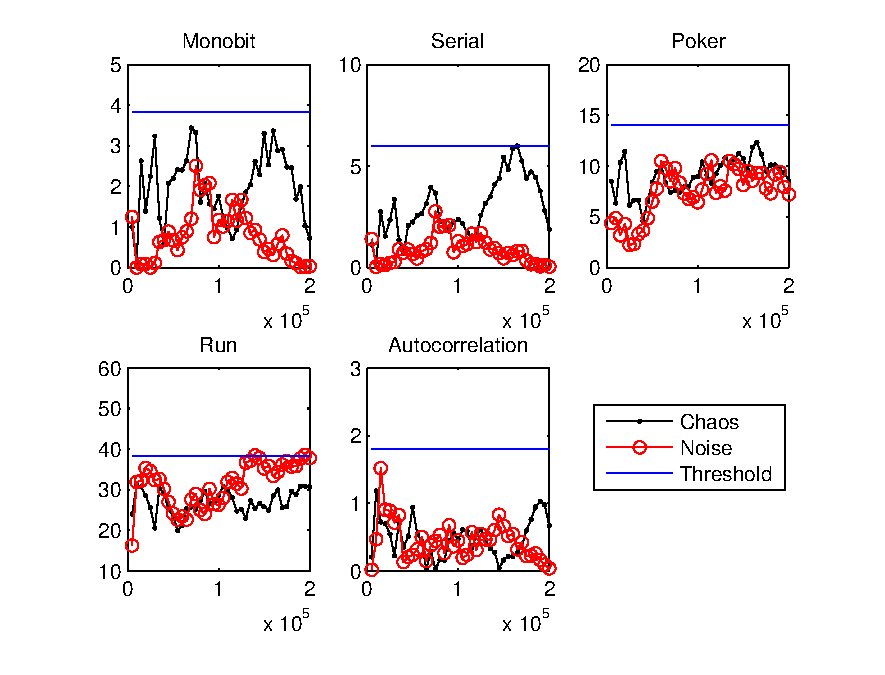
\includegraphics[width=1\textwidth]{comparison.eps}}
  \subfigure[$20$GHz, $4$th DSD, and $8$ LSB
  method]{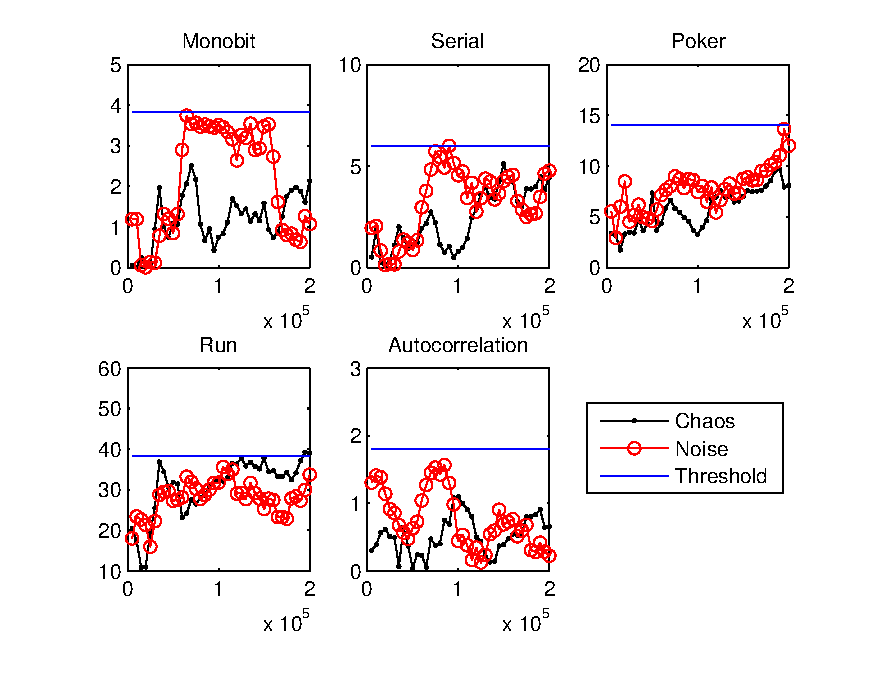
\includegraphics[width=1\textwidth]{comparison2.eps}}
  \hspace{0.5cm}
  \caption{Overall Sequence Stability Comparison}
  \label{fig:Comparison2}
\end{figure}

Finally a comparison of the overall stability from $5\times10^3$ to
$2\times10^5$ for these generators is given in
Fig.\ref{fig:Comparison2}. It can be seen that the trends for the
amplitude movements of values are more or less in the same scale,
which again indicates that all these random sequences share closed
random properties.
%
\begin{table*}[!t]
  % \begin{small}
  \centering
  \renewcommand{\arraystretch}{1.3}
  \caption{Comparison between the presented sources for a $2 \times 10^7$ bits sequence}
  \label{Comparison}
  \centering
  \begin{tabular}{|c|c|c|c|c|c|}
    \hline
    \textbf{Subjects} & Monobit & Serial & Poker & Runs & Autocorrelation  \\ \hline
    Method& \multicolumn{5}{c|}{ $2.5$GHz, $1$st DSD, $5$LSBs}\\ \hline
    Chaotic laser  		&0.2509	&1.9200	&16.6650&16.6215&1.5739\\ 
    Noise 	&0.6019	&0.7144	&8.5606&17.5156&1.5247\\ \hline
    Method &\multicolumn{5}{c|}{ $20$GHz, $4$st DSD, $8$LSBs}\\ \hline
    Chaotic laser  		&1.4580	&0.5199	&13.1430 &28.9460 &1.1583\\
    Noise 	&0.2554	&0.7835	&14.0035&22.9136&1.6739\\ \hline
    
    \hline
  \end{tabular}
  % \end{small}
\end{table*}

\section{Discussion, Conclusion, and Perspectives}
\label{conclusion}
Random number generation via photonic broadband signal generation does
provide nowadays a novel and interesting approach allowing for
unprecedented high bit rate of random bit streams. These photonics to
digital world conversion are designed so that randomness can be
certified according to most of the usual randomness tests such as NIST
and DieHARD suites. Among the recently proposed physical systems and
related processing intended to extract bit streams from photonic
analogue waveforms, two rather different approaches can be identified:
when the source of randomness explicitly stems from photonic noise
\cite{li:OL11,wetzel:ox12}, and when deterministic chaos is claimed to
be at the origin of the random bit stream
\cite{fast,ultrafast2009}. Whereas the first approach provides
obviously, and by definition, a non deterministic random bit stream,
the second one has an implicit source of determinism, similarly to the
algorithmic and fully digital pseudorandom bit sequence (PRBS)
generators.\\ A major interest of the digital PRBS resides in their
capability of generating a distant and synchronized random bit stream,
which allows one to apply them in symmetric cryptography. A major
advantage of PRNG is precisely their perfect determinism, and perfect
control, due to their digital program-based generation process. This
feature is also at the origin of their main drawback: the same
absolute digital determinism can be used in principle for
cryptanalysis, trying to guess the seed which can then
deterministically and totally allow for the random bit sequence
reproduction, even by an eavesdropper. Also from a more technical
viewpoint, the processor based architecture of PRNGs defines some
speed limitations related to the processor clock, and the number of
elementary operations needed to implement the PRNG algorithm. Noise
based, and chaos based, photonic RNGs provide at least a technical
answer to the limited bit rate generation provided by purely
algorithmic solutions. It was also reported in many attempts on
photonics based RNGs, that high quality randomness is possible, since
they can pass successfully all the standard NIST and DieHARD test
suites. A strong open problem however still remains concerning the
capability to control, and reproduce, the random bit stream provided
by photonic chaos-based RNGs. On the contrary to the photonic noise
based RNGs, this indeed can be expected from the chaos-based photonic
RNGs, since they also originates, at least partially, on deterministic
dynamics, similarly to the algorithmic PRNGs.\\ In that particular
context, we have proposed in this article to address related issues,
through an analysis of the deterministic origin of the chaos-based
photonic RNGs proposed in \cite{ultrafast2009}. Indeed, a major
difference between purely digital PRNGs and photonic chaos-based RNGs
resides in the presence of unavoidable non-deterministic noise
sources. This noise compound can be used as an argument to support the
idea that one might find an ``analogue protocol'', such that a
non-authorized receiver would never be able to reproduce the bit
stream. This would then lead to an absolutely secure symmetric
cryptographic scheme, e.g. if the Vernam cipher scheme is
employed. Before reaching this absolute dream of secure
communications, one has however to clearly identify how deterministic
the final random bit stream, or differently speaking, how far any
deterministic mechanism indeed does exist in this bit stream so that
one can think about using it to reproduce the random bit stream. This
is one of the main point addressed in this chapter, in the particular
context of the method proposed in
\cite{ultrafast2009}.\\
The particularity of this method, is that it combines both photonic
chaos, but also a significant digital post-processing before the
extraction of a final bit stream with excellent randomness. We have
reproduced in this chapter this method on other photonic sources of
analogue entropy. One is consisting in a mainly deterministic
electro-optic phase chaos generator, a broadband chaos generator
recently used to demonstrate the currently fastest analogue chaos
based communication scheme. Determinism in this photonic chaos setup
can be claimed as a dominating feature, since it was used and
controlled to achieve a field experiment of chaos communication at
10~Gb/s. On the contrary, another photonic source of entropy was also
considered in the same photonic RNG method. This second photonic
source of entropy can be trustfully considered as of mainly noisy
origin, without any deterministic and controllable compound: its
origin is typically attributed to intrinsic diode laser RIN (relative
intensity noise), photodiode detection noise, and electronic
amplifiers noise. We found that the method proposed in
\cite{ultrafast2009} gave fully comparable results in terms randomness
quality of the generated bit stream. This is fully consistent with the
questioning already addressed in \cite{williams:OE10,hirano:OE10}
about the actual origin, noise or chaos, of the random bit stream
provided by this method. Additionally to this result, we have proposed
analysis of this method on the basis of standard signal theory and
sampling theory. The conclusion of our analysis strongly support that
the method is essentially exploiting the noisy compound always present
in a photonic signal, would it be with (chaos) or without (noise)
deterministic motion. Our analysis has highlighted in the
post-processing bit extraction method, two dominating mechanisms
leading to a high quality random bit stream. One is related to the
natural spectral mixing occurring when aliasing is involved. In the
acquisition method proposed in \cite{ultrafast2009}, an undersampling
of a factor 16 is indeed performed, which is equivalent to a strong
aliasing condition in the photonic samples extraction. This aliasing
phenomenon definitely enhances the randomness quality of the original
signal (would it be of chaotic or noisy origin), through its well
known complex amplitude mixing in the Fourier domain. Another
post-processing which we have called DSD for distant sample
difference, was also shown to contribute to the randomness quality of
the final bit stream. Combined together with an LSBs retaining only,
we showed numerically that the final bit stream appears to be
extracted from a nearly uniform probability distribution of the
amplitudes corresponding to the retained LSBs. The LSB retaining
procedure also obviously gives an important role to the small
amplitudes which are mainly dominated by noise sources, whereas MSB
are of course more correlated with large amplitude deterministic
motion. To develop an evidence of the actually most important role of
the noise instead of the deterministic chaotic motion, we have
proposed to analyze the binary entropy rate for each selected bit,
from LSB to MSB, without or with one or several DSD
post-processing. The existence of a non zero memory time was found
only for large amplitude bits (close to MSB), and for a small number
of DSD post-processing. This configuration which reveal a signature of
the deterministic origin via the evolution of the binary entropy, is
the opposite one with respect to the choice proposed in
\cite{ultrafast2009}. It thus confirms that negligible deterministic
origin (and thus the chaotic light motion) actually enters in the
randomness of the final bit stream.

Using the MSB (or equivalently 1-bit ADC conversion) is according to
us the way to keep a deterministic origin in the generation of a
random bit sequence. Further work on ultra-fast RNGs based on
deterministic chaos, should thus concentrate on this approach for the
bit extraction method from the original photonic chaotic
waveform. Careful post-processing will however be very important, to
ensure that randomness quality is indeed obtained though strong
determinism is concerned. In \cite{fast}, this was achieved through
the use of two independent chaotic lasers, with careful chosen
resonant frequency and external cavity delayed feedback, and a XOR
operation between their respective 1-bit ADC. Finally, the most
difficult task will be to design a proper coupling scheme with a
binary bit stream, so that distant random sequences can be
synchronized and used for cryptography.





\chapter{CI Random Stream Generation Via Optoelectronic Chaotic Laser}
\label{CI Random Stream Generation Via Optoelectronic Chaotic Laser}

According to the analysis of the previous chapter, MSB is a key factor to preserve
 the deterministic origin in the generation of random streams using optoelectronic
chaotic lasers. Since the MSB keeps the most large part of information on the chaotic laser signal, the statistical performance of the extracted output bit stream is not good.
Hence, in this chapter, we will try to use the method based on chaotic iterations
and presented in previous chapters to fulfill this drawback.
% From the description of~\cite{bfg12a:ip} (Chapter~\ref{An optimization technique on pseudorandom generators based on chaotic iterations}), CI
Indeed, this method has been able to improve the statistical properties of
various defectives PRNGs, thus we think interesting to regard weather this
approach can work too for chaotic laser based pseudorandom generation.

%\section{CI method}
\section{Setup of a broadband optoelectronic chaotic laser signal}

We have presented in the previous part of this manuscript 5 generators based on 
chaotic iterations, namely the four versions of CIPRNG, and the XOR CI generator 
proposed in~\cite{DBLP:journals/corr/abs-1112-5239}, which is a GPU adaptable 
version of the aforementioned CI methods. 
These schemes are not only able to assign discrete chaotic properties to the output streams, but the statistical properties of the generators set as parameters are also improved.
This is why we tried to use them on an optoelectronic device similar to the
one studied in the previous chapter.

\begin{figure}
\centering
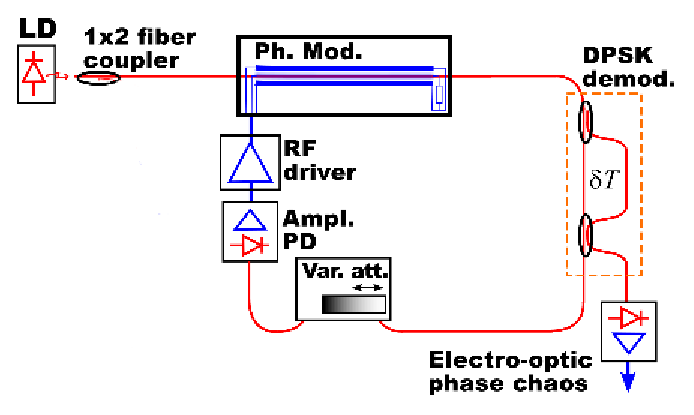
\includegraphics[scale=0.8]{setup_opto_laser.eps}
\caption{chaotic laser signal setup}
\label{chaotic laser signal}
\end{figure}
%\section{Setup of a broadband optoelectronic chaotic laser signal}
Indeed, as shown in Fig.~\ref{chaotic laser signal}, the chaotic laser signal considered
in this chapter is similar to the one described in Section~\ref{Method for random bit sequence generation}, except that there is no output signal for photonic noise. 
This physical source of entropy presents a very strong determinism. 
The output chaos signal is generated by a nonlinear dual delay differential 
equation implemented in an optoelectronic and electro-optic feedback loop.

\section{Random stream generation approach by applying CI method to chaotic laser}

In this section, a last structure for random sequence generation is presented: the optoelectronic chaotic laser is post-processed by using chaotic iterations.
Two examples are then shown and the NIST test suite is used to evaluate 
the produced outputs.

\subsection{The proposed scheme}
\begin{figure}
\centering
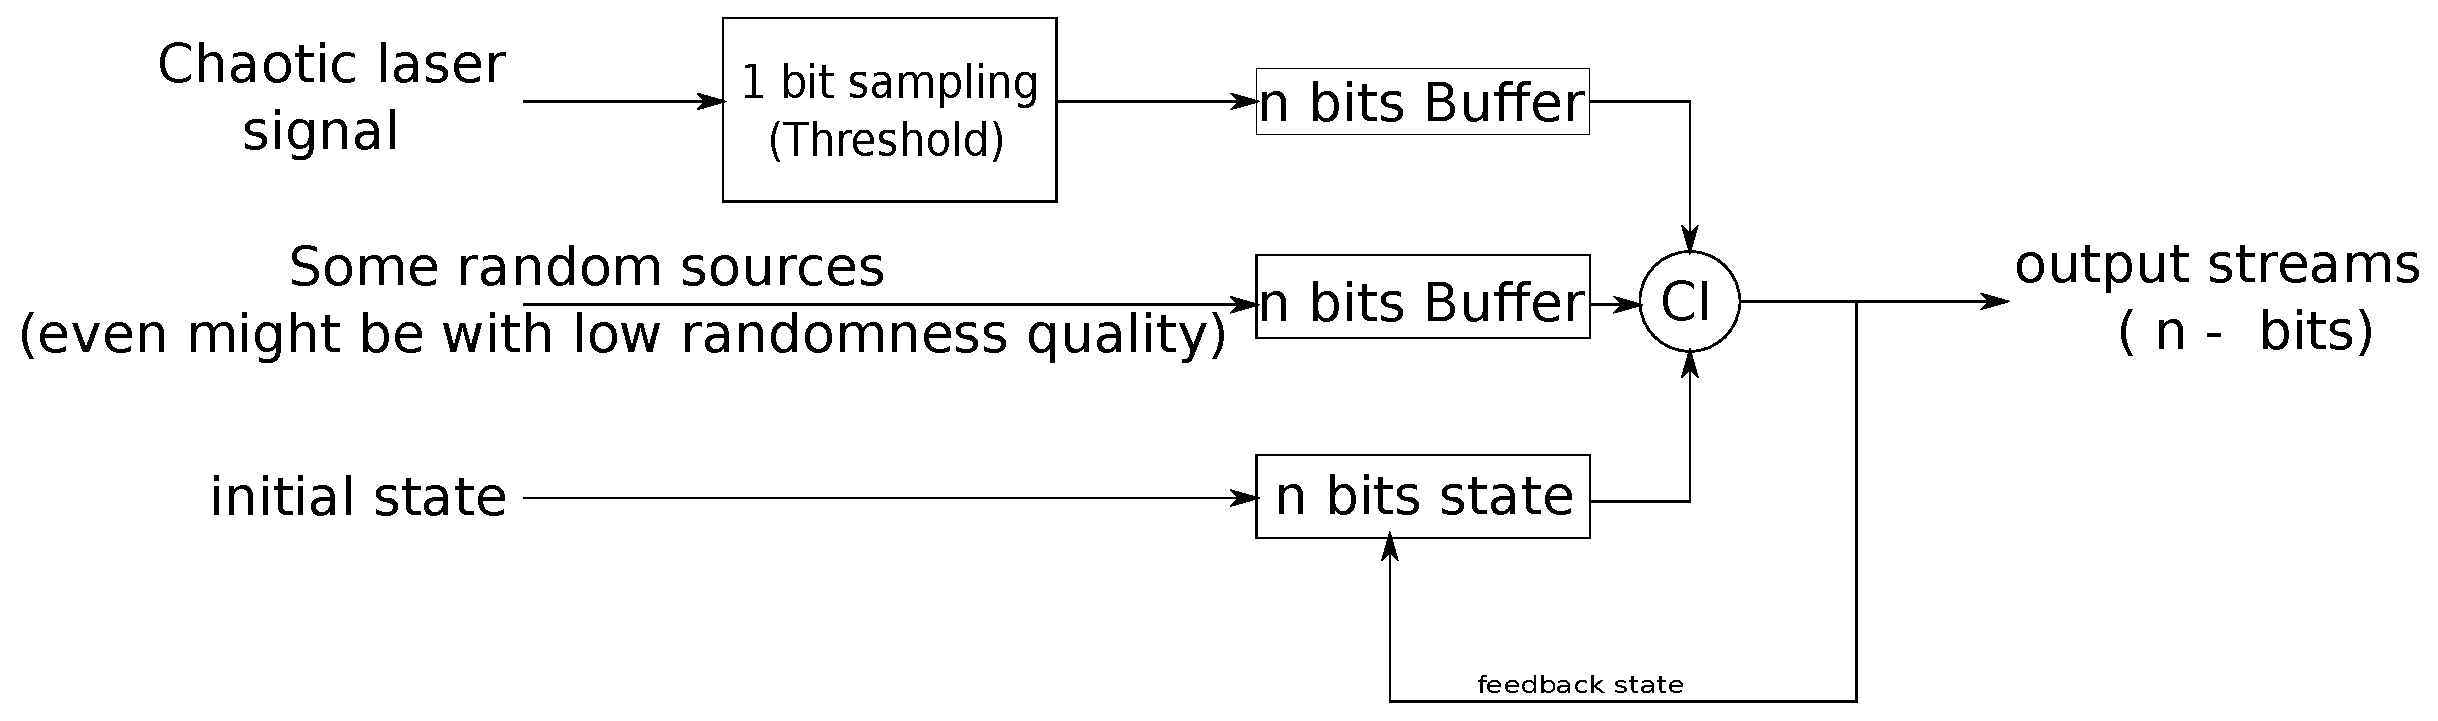
\includegraphics[scale=0.3]{CI_Photononic.eps}
\caption{The scheme of applying CI to chaotic laser}
\label{The scheme of applying CI to chaotic laser}
\end{figure}

%The scheme of adapting CI to chaotic laser is represented here.
For achieving randomness, three different inputs are used and mixed using
the chaotic iterations post-processing:
\begin{itemize}
\item the chaotic laser sampled to 1-bit (collected as $n$-bits integer using a buffer),
\item another given (pseudo)random source to determine (producing $n$-bits values),
\item and the current state of the system. 
\end{itemize}
As depicted in Fig.\ref{The scheme of applying CI to chaotic laser}, the chaotic laser 
signal is sampled by a 1-bit ADC. The sampling rule consists to compare the voltage of 
the chaotic laser signal with a threshold value: if the voltage is bigger than the
threshold, then the output bit is $1$, else it is $0$. 
This binary stream provided by a 1-bit sampling of the chaotic laser cannot exhibit 
a good statistical profile, as a lot of ``chaos information'' is lost during the sampling.
This is why we propose to employ two other inputs, namely
another (pseudo)random number source and the current state 
of the iterated system. As shown in Fig.\ref{The scheme of applying CI to chaotic laser},
these two inputs are mixed with the chaotic laser binary stream using 
chaotic iterations. Each $n$-bits values obtained by this way is 
both returned as output of the device and reused in the next iteration
of the system.

\subsection{Examples of processing}

Examples are given in this subsection by using two usual generators as random source input: XORshift and LFSR (Linear Feedback Shift Register \cite{beker1982cipher}). 
They have been chosen due to their rapidity and very simple design,
making them easy to implement in hardware. 
The CI method is a modified version of the XOR CI generator presented in \cite{DBLP:journals/corr/abs-1112-5239}. 
In the next section, we give a brief description about this new XOR CI generator, 
we define the LFSR and recall the XORshift PRNGs for easy reading of this manuscript, and we provide  the parameters  of the laser setup.

\subsubsection{A new XOR CI generator}

As recalled previously, the XOR CI method is one way to use chaotic iterations
as PRNGs~\cite{DBLP:journals/corr/abs-1112-5239}. Compared to the other CIPRNG schemes, 
XOR CI is very compatible in physical design. In XOR CI, at each iteration, a subset of
binary digits from the output value of a PRNG is chosen to be switched, this subset
depending on the value of a second generator. 
Such an attempt leads to a sort of merger of the tow sequences. 
Our XOR CI algorithm only consists in adding the chaotic signal
provided by the laser into his process.
The corresponding algorithm can be written as follows.

\begin{algorithm}
\textbf{$Input$:} the internal state $x$ (an array of 4-bit words)\\
\textbf{$Output$:} an array $r$ of 4-bit words
\begin{algorithmic}[1]
\STATE$b\leftarrow{Chaotic\_Laser\_data()}$;
\STATE$a\leftarrow{PRNG_1()}$;
\STATE$x = x \oplus a \oplus b$;
\STATE$r\leftarrow{x}$;
\STATE return $r$;
\medskip
\caption{An arbitrary round of the respective XOR CI generator}
\label{XOR CI}
\end{algorithmic}
\end{algorithm}

For $PRNG_1$, we will use XORshift and LFSR in our simulations; they are recalled below.

\subsubsection{XORshift}
The definition of this well-known generator is reminded again in Algo.\ref{aaaaaaa}: 
\begin{algorithm}
\textbf{Input:} the internal state $z$ (a 32-bits word)\\
\textbf{Output:} $y$ (a 32-bits word)
\begin{algorithmic}[1]

\STATE$z\leftarrow{z\oplus{(z\ll13)}}$;
\STATE$z\leftarrow{z\oplus{(z\gg17)}}$;
\STATE$z\leftarrow{z\oplus{(z\ll5)}}$;
\STATE$y\leftarrow{z}$;
\STATE return $y$\;
\medskip
\caption{An arbitrary round of XORshift algorithm}
\label{aaaaaaa}
\end{algorithmic}
\end{algorithm}

\subsubsection{LFSR}
In computing, LFSR is a shift register whose input bit is a linear function of its previous state. The most commonly used linear function of single bits is XOR. Thus, a LFSR is most often a shift register whose input bit is driven by the exclusive-or (XOR) of some bits of the overall shift register value. This generator, 
described Algo.\ref{bbbbb}, has a period equal to $65535$.

\begin{algorithm}
\textbf{Input:} the internal state $z$ (a 16-bits word, set as $0xACE1$ initially )\\
\textbf{Output:} $y$ (1 bit)
\begin{algorithmic}[1]
\STATE$y = ((lfsr \gg 0) ^ (lfsr \gg 2) ^ (lfsr \gg 3) ^ (lfsr \gg 5) ) \& 1$;
\STATE$z = (z \gg 1) | (bit \ll 15)$;
\STATE return $y$\;
\medskip
\caption{An arbitrary round of LFSR algorithm}
\label{bbbbb}
\end{algorithmic}
\end{algorithm}


\subsubsection{Photonic chaos}
For experiments purpose, a chaotic laser has been stimulated in computer using 
the method detailed in~\cite{PhysRevE.79.026208}. The frequency of the signal is
equal to $F_1 = 4000$ GHz, and other corresponding parameters are listed as:
\begin{itemize}
 \item \textbf{Time delay}: Set XORshift as $60$ns;
 \item \textbf{High Frequency Cut-off}: $13$ps;
 \item \textbf{Ratio between high and low frequency cut-off}: $5\times10^{-5}$;
 \item \textbf{Type of nonlinear transformation}: square of sinus;
 \item \textbf{Highest complexity chaotic regime}: 5.
\end{itemize}
When the laser data are being processed, one value every $400$ is selected to be $1$-bit sampled ($10$ GHz). Since the output of XORshift PRNG is in $32$ bits, thus we have $n = 32$
in Fig.\ref{The scheme of applying CI to chaotic laser}.

\section{NIST test results}
The randomness of the output streams of these two simulated examples are evaluated by 
the standard NIST test suite. The results are shown in Tab.\ref{nist ci chaotic laser}. 
We can see that, if no CI is applied,  the chaotic laser sampled 
bits cannot pass the battery. As usual, the generator XORshift fail one test. 
And none can be passed for LFSR, since this generator has a very low period. 

With the chaotic iteration based post-treatment referred as CI method, the performances 
 have been improved obviously (see Table~\ref{nist ci chaotic laser}). 
We can conclude that, even though the participated random sources are not as good as possible, the CI method still remains to be able to improve the statistical properties of the inputted 
generators.

\begin{table*}[!t]
  \renewcommand{\arraystretch}{1.3}
  \caption{NIST SP 800-22 test results ($\mathbb{P}_T$)}
  \label{nist ci chaotic laser}
  \centering
  \begin{tabular}{|l|c|c|c|c|c|c|}
    \hline
    Method & CI with  & XORshift &  CI with & LFSR & No CI  \\ 
           & XORshift &          &  LFSR   &       &         \\\hline\hline
    FT 	&  0.935716 &  0.14532 & 0.12414&  0.000000&  0.171867  \\ \hline
    FBT 	 & 0.040108 & 0.45593 & 0.73425& 0.000000&  0.289667 \\ \hline
    CST 	&  0.334152 & 0.21330 &  0.000000& 0.000000&  0.000000 \\ \hline
    RT 	&  0.595549 &  0.28966 & 0.88330&  0.000000&  0.000000 \\ \hline
    LROBT 	 & 0.191687 &  0.000000 & 0.01245& 0.000000&  0.000000 \\ \hline
    BMRT 	 & 0.534146 &  0.005350 & 0.42803&  0.000000&  0.000000 \\ \hline
    FFT: 	 & 0.236810 &  0.50365 &0.33157 &  0.000000&  0.000000 \\ \hline
    NOTMT	&  0.502510 &  0.86769 &0.51246 &  0.000000&  0.000000 \\ \hline
    OTMT 	&  0.851383 &  0.27570 &0.01235 &  0.000000&  0.090936 \\ \hline
    MUST 	  &0.798139 &  0.92407 & 0.81246& 0.000000&  0.000000 \\ \hline
    AET &	  0.224821 &  0.75792 &0.00000 & 0.000000&  0.000000 \\ \hline
    RET 	&  0.347389 &  0.41902& 0.91235 &  0.000000&  0.471174 \\ \hline
    REVT &	  0.217344 &  0.81154 &0.12592 &  0.000000&  0.461569 \\ \hline
    ST	 & 0.300289 &  0.41923 &  0.000000& 0.33122 & 0.237996\\ \hline
    LCT &	  0.350485 &  0.52833 &0.81245&  0.000000&  0.224821\\ \hline
Success 			&15/15		&14/15 &13/15	 &0/15		&7/15 \\ \hline
  \end{tabular}
\end{table*}



%\section{Conclusion}
As suggested by these short experiments, the combination of chaotic laser and our CI method 
%is attempted in this chapter. As we can see, 
%CI method 
may lead to statistical improvement of the physical signal. 
If these results are confirmed by further investigations, such a way 
to proceed may provide an interesting way to produce physically no periodic
reproducible, ultra fast, and chaotic random streams with good statistical profiles.

 
